\documentclass[a4paper, oneside,11pt]{article}
\usepackage[a4paper,top=3cm,bottom=3cm,left=3cm,right=3cm,marginparwidth=1.75cm]{geometry}
\usepackage[utf8]{inputenc}
\usepackage{lipsum}
\usepackage{graphicx}
\usepackage{times}
\usepackage{xcolor}
%\usepackage{booktabs}
\usepackage{float}
\usepackage{color}
\usepackage{hyperref}
\usepackage{amsmath}
%\usepackage{subfig}
\usepackage{subcaption}
\usepackage[backend=biber,
    style=numeric,sorting=none]{biblatex}
\addbibresource{ref.bib}
\hypersetup{
    colorlinks=true,
    linkcolor=blue,
    urlcolor=blue,
}
\graphicspath{{/}}
\usepackage{adjustbox}
\usepackage{tabularx}
\usepackage{multirow}
\usepackage{titlesec}
\usepackage{graphicx}
\usepackage{upgreek}
\usepackage{enumitem}  
\usepackage{comment} 
\usepackage{upgreek}
%%%%%%%%%%%%%%%%%%%%%%%%%%%%%%%%%%%%%%%%%%%%%%%%%%%%%%%%%%%%%%%%%%%%

\begin{document}

\begin{table}[h]
		\begin{adjustbox}{width = \linewidth}
			\begin{tabular}{c c c}
				\multirow{5}{*}{ 
\includegraphics[width=0.13\textwidth]{iitb_logo.png}} \hfill &  \large{{Student Satellite Project}}  & \hfill \multirow{5}{*}{ 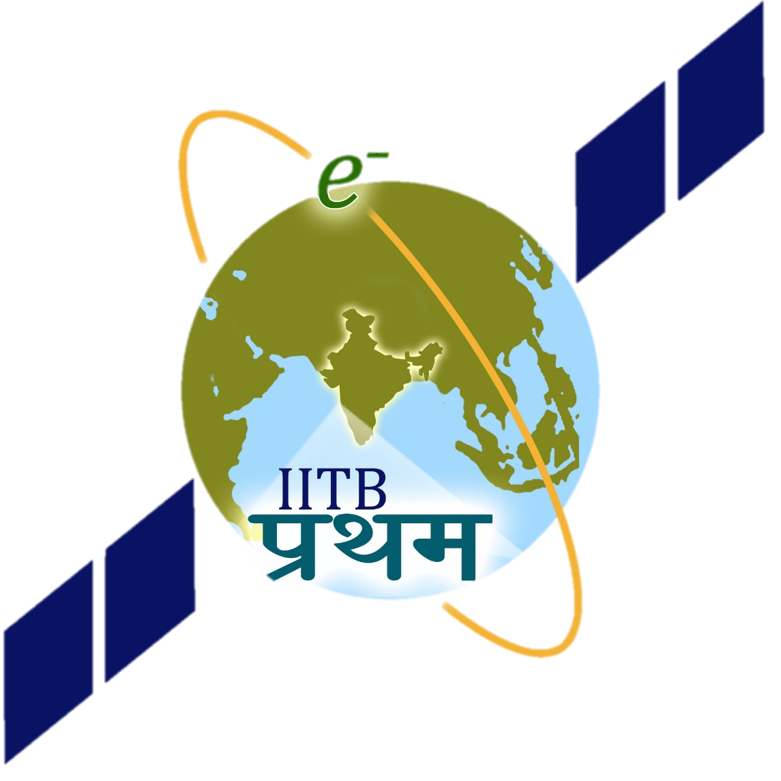
\includegraphics[width=0.13\textwidth]{pratham_logo.png}} \\
				& {Indian Institute of Technology, Bombay} &\\
				& {Powai, Mumbai - 400076, INDIA} &\\
				&{} &\\
				& Website: {www.aero.iitb.ac.in/satlab} &\\
				\\
				&\large{\textbf{Readme file for getOrbitData.py}}&\\
				&Attitude Determination and Control Subsystem&\\
				\hline
			\end{tabular}
		\end{adjustbox}
\end{table}
\section*{filename}
\textbf{Author:Sumit Agrawal}\\
\textbf{Date:06 October 2018}\\
This function takes orbital elements and calls sgp\_fn, to generate position and velocity of satellite at different time instants.\\
Input:TT - Total time of the orbit in minutes\\
MS - Model step time (MODEL\_STEP - step size in environmental data in seconds
)\\		
MeanMo - Mean motion in revolution per day\\
Eccen - Eccentricity\\
Incl\_deg - Inclination in degrees \\
MeanAnamoly\_deg - Mean Anamoly in degrees \\
ArgP - Argument of perigee in degrees \\
RAAN\_deg - Right ascension of ascending node in degrees\\
sgp\_output - timestep, position and velocity in second, meter and meter per second respectively.\\ getOrbitData\_TLE or getOrbitData\_OrbitELement give would be used to create this file.\\ 
Output: sgp\_i\_TT$\%g\_MS\%g_MMo\%g\_Ecc\%g\_Incl\%g\_MAnamoly\%g\_ArgP\%g\_Raan\%g.csv
$\\
example : sgp\_i\_TT100\_MS0.1\_MMo16.0582\_Ecc0.0086731\_Incl72.8435\_MAnamoly110.571 \\
\_ArgP52.6988\_Raan115.969
\\
\\
\textbf{Note}: There are two functions to generate the csv file one is  getOrbitData\_TLE and another is  getOrbitData\_OrbitElement.  Use getOrbitData\_TLE when you want to give the input to the sgp function as Two Line Element (TLE). Since for simulation and testing purposes creating TLE data is quite cumbersome so getOrbitData\_OrbitElement function is written to generate sgp files directly from orbital elements. The orbital elements required to csv file of sgp is mentioned in the description of the function below.

\section*{getOrbitData\_TLE}
\textbf{Author:Sumit Agrawal}\\
\textbf{Date:06 October 2018}\\
Objective of getOrbitData function is to take relevant input such as either TLE or orbital elements from constants\_1U.py and fed it to sgp\_fn to create trajoctory of satellite. In other words position and velocity of satellite in ECI frame at each timesteps.

Sometime we know TLE data (like from n2yo.com) and want to create orbit in that case this getOrbitData\_TLE can be used to call sgp\_fn.
This function also call TLE2OrbitElements as sgp function require input in terms of orbital elements.TLE2OrbitElements converts TLE into orbital elements.
Input:TT - Total time of the orbit in minutes\\
MS - Model step time (MODEL\_STEP - step size in environmental data in seconds
)\\
dT - time vector from the constant.py\\
MS - Model step time from the constant.py.\\ 
Output:sgp\_output.csv (Position and velocity of satellite in ECI frame in m and m/s). It also call filename function for naming of sgp\_output in terms of orbital elements of the starting point.  \\
\\ 
\\
\section*{getOrbitData\_OrbitElement}
\textbf{Author:Sumit Agrawal}\\
\textbf{Date:06 October 2018}\\
 This function takes orbital elements directly from constants\_1U.py and calls sgp\_fn to generate orbit.  \\
Input:TT - Total time of the orbit in minutes\\
MS - Model step time (MODEL\_STEP - step size in environmental data in seconds
)\\
MeanMo - Mean motion in revolution per day\\
Eccen - Eccentricity\\
Incl\_deg - Inclination in degrees \\
MeanAnamoly\_deg - Mean Anamoly in degrees \\
ArgP - Argument of perigee in degrees \\
RAAN\_deg - Right ascension of ascending node in degrees\\
sgp\_output - timestep, position and velocity in second, meter and meter per second respectively. Output:sgp\_output.csv (Position and velocity of satellite in ECI frame in m and m/s). It also call filename function for naming of sgp\_output in terms of orbital elements of the starting point.  \\
\\
\\
References:
\href{https://en.wikipedia.org/wiki/Two-line_element_set}{Two line Element} \\
\href{https://www.celestrak.com/NORAD/documentation/spacetrk.pdf}{Celestrak SGP report}\\
\href{https://en.wikipedia.org/wiki/Simplified_perturbations_models}{Simplified General Perturbation model}\\
\href{https://www.n2yo.com/satellite/?s=41783#results}{N2YO website to get TLE of any space object}
\printbibliography 
\end{document}
